\section{Failure of Intrusive Linear ROMs}

To begin, linear subspace MP-LSVT PROMs are tested. The primitive trial basis is computed from the concatenated training datasets (accounting for 18,009 snapshots), centered about the time-average mean of the dataset and normalized by min-max scaling. Details on this centering and scaling operation can be found in Section~\ref{sec:centerScale}. For a given forcing frequency, the PROM is restarted from the corresponding primitive state snapshot at $\timeVar = 75 \mu$s and allowed to run for 20,000 iterations with a time step of $\dt = 25$ ns.

\begin{figure}
    \begin{minipage}{0.49\linewidth}
        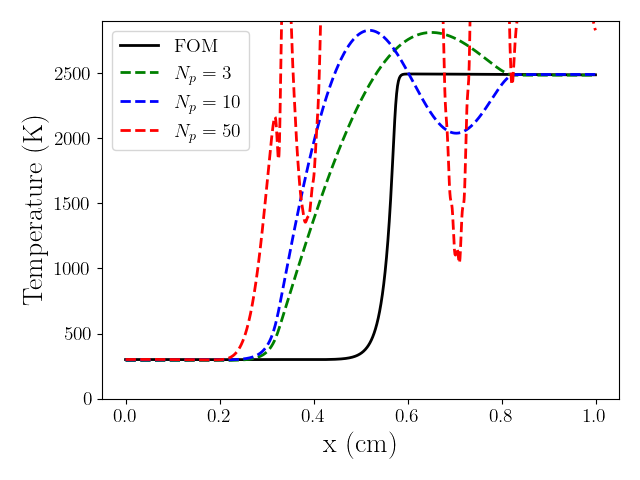
\includegraphics[width=0.99\linewidth]{Chapters/TransientFlame/Images/linear/rom_temp_snaps.png}
    \end{minipage}
    \begin{minipage}{0.49\linewidth}
        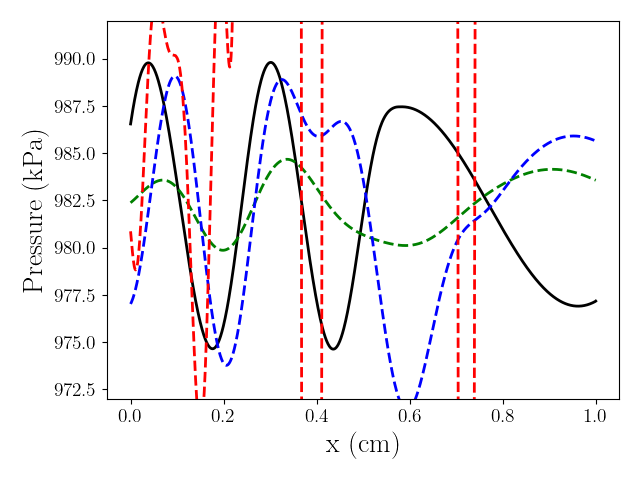
\includegraphics[width=0.99\linewidth]{Chapters/TransientFlame/Images/linear/rom_press_snaps.png}
    \end{minipage}
    \caption{\label{fig:flameLinearROM}Intrusive linear subspace MP-LSVT PROM temperature (left) and pressure (right) snapshots, various $\numPrimModes$.}
\end{figure}

Unfortunately, all linear subspace PROMs performed abysmally for all forcing frequencies. This can be plainly seen in Fig.~\ref{fig:flameLinearROM}, where low trial space dimensions (here, $\numPrimModes = 3, \; 10$) results in smeared gradients and decoherence of the pressure signal. At higher trial space dimensions ($\numPrimModes = 50$), the solution is entirely unstable, devolving into a meaningless flow field. 

\begin{figure}
    \begin{minipage}{0.49\linewidth}
        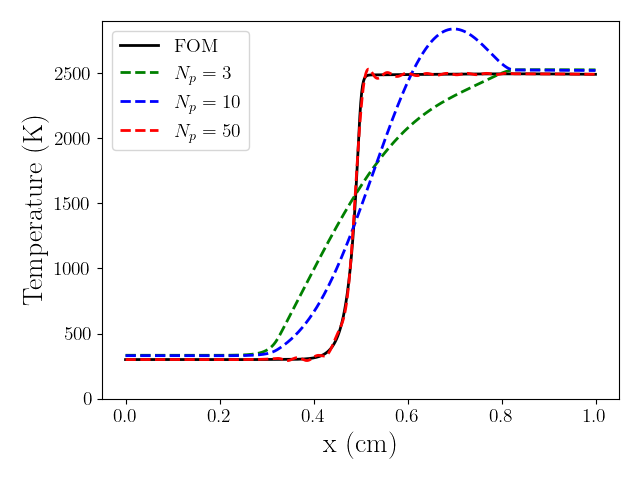
\includegraphics[width=0.99\linewidth]{Chapters/TransientFlame/Images/linear/proj_temp_snaps.png}
    \end{minipage}
    \begin{minipage}{0.49\linewidth}
        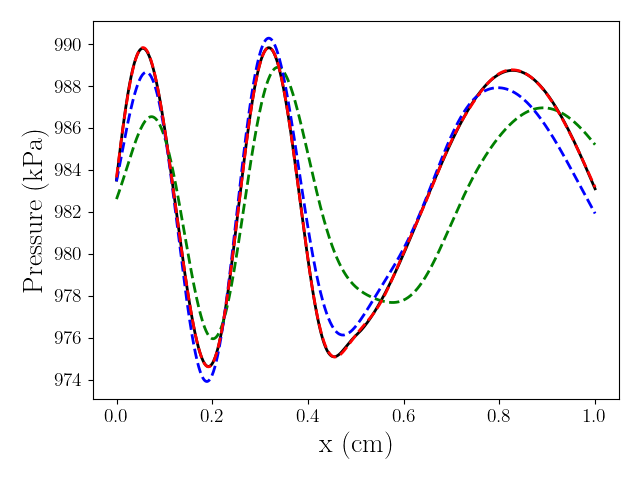
\includegraphics[width=0.99\linewidth]{Chapters/TransientFlame/Images/linear/proj_press_snaps.png}
    \end{minipage}
    \caption{\label{fig:flameLinearProj}Linear projections of temperature (left) and pressure (right) fields, $f = 150$ kHz, various $\numPrimModes$.}
\end{figure}

The primary reasons for these failures can be observed from the linear projection of the solution onto the trial space. Figure~\ref{fig:flameLinearProj} shows the projected temperature and pressure fields. For the temperature field, which experiences a strong gradient at the flame, a linear representation will invariable result in significant under- and overshoots in the vicinity of the jump. Increasing the trial space dimension decreases the magnitude of these overshoots but gives rise to high-frequency ``ringing'' behavior near the flame. This is similar to the Gibbs phenomenon observed in approximating discontinuities with a Fourier series. The accuracy of the projected pressure field is similarly poor, though given the relatively smooth nature of this field, increased trial basis resolution converges to an accurate approximation without visible discrepancies.

The poor performance of linear subspace PROMs in modeling advection-dominated flows with strong gradients comes as no surprise, given the previous discussion of slowly-decaying Kolmogorov $n$-widths in in Section~\ref{subsec:nonlinManifold}. Non-linear alternatives are explored next, in an attempt to alleviate these issues.